\documentclass[10pt,twocolumn]{article}
	
\usepackage{myfontstyle}
\usepackage{mypackages}
\usepackage{mymacros}
\usepackage{mycommands}
\usepackage{graphicx}
\usepackage{hyperref}

\begin{document}
\thispagestyle{fancy1}

%%% Title and Abstract------------------------
\twocolumn[
\begin{center}
	\hrule
	\vspace{3pt}
	% Title:
	{\sffamily\bfseries\Large
		Report for Assignment 8: Convolutional Neural Network Shelf Inspector
	} \\
	{\color{gray}
		\vspace{3pt}
		\hrule
		\vspace{3pt}
	}
	{
		\hspace*{\fill}
		Julian Soh
		\hspace*{\fill}
%		Second Author
%		\hspace*{\fill}
%		Third Author
%		\hspace*{\fill}
%		Fourth Author    % uncomment these two lines if there's a fourth author
%		\hspace*{\fill}
	}\\
	\vspace{3pt}
	{\itshape
		\hspace*{\fill}
		Department of Mechanical Engineering, Saint Martin's University
		\hspace*{\fill} \\
		\hspace*{\fill}
		ME/EE 467---Machine Intelligence
		\hspace*{\fill}
	}\\
	\vspace{3pt}
	{
		\hspace*{\fill}
		\today{} % today's date ... can type manually instead
		\hspace*{\fill}
	}
	\vspace{3pt}
	{\color{gray}\hrule}
%	\vspace{2pt}
\end{center}
% Abstract:
\begin{adjustwidth}{1.5in}{1.5in}
{\small
\noindent\textbf{Abstract.} \hspace{1em}
Build, train, and evaluate a convolutional neural network (CNN) for classifying warehouse shelf images into three categories (normal, damaged, overloaded) and applying the full regularization toolkit.
}
\end{adjustwidth}
\vspace{9pt}
\hrule
\vspace{1\baselineskip}
]

%%% Body -------------------------

\section{Introduction} 
\label{sec:introduction}

Convolutional neural networks (CNNs) can be used to learn spatial hierarchies of features from images. This report demonstrates how CNNs are used in classifying warehouse shelf images into three categories: normal, damaged, and overloaded.

A dataset containing images of warehouse shelves is used. This dataset contains patterns that a linear model cannot capture, while a CNN can learn these complex spatial relationships and make accurate predictions.

\section{Methods}

\subsection{Build and Train a CNN}
We implemented a 3-block convolutional neural network in PyTorch:

\begin{itemize}
	\item \textbf{Conv block 1:} \texttt{Conv2d(1\,$\rightarrow$\,16, kernel\_size=3, padding=1)} $+$ ReLU $+$ \texttt{MaxPool2d(2)}
	\item \textbf{Conv block 2:} \texttt{Conv2d(16\,$\rightarrow$\,32, kernel\_size=3, padding=1)} $+$ ReLU $+$ \texttt{MaxPool2d(2)}
	\item \textbf{Conv block 3:} \texttt{Conv2d(32\,$\rightarrow$\,64, kernel\_size=3, padding=1)} $+$ ReLU $+$ \texttt{MaxPool2d(2)}
	\item \textbf{Classifier:} \texttt{Flatten} $\rightarrow$ \texttt{Linear(64*8*8, 128)} $+$ ReLU $\rightarrow$ \texttt{Linear(128, 3)}
\end{itemize}

The spatial resolution is reduced as 64$\times$64 $\rightarrow$ 32$\times$32 $\rightarrow$ 16$\times$16 $\rightarrow$ 8$\times$8, and the model outputs 3 classes. For multiclass prediction, the output scores (logits) $\mathbf{z}=(z_1,\ldots,z_K)^\top$ are interpreted with softmax,
\[
\hat{y}_k = \mathrm{softmax}(z_k) = \frac{e^{z_k}}{\sum_{j=1}^{K} e^{z_j}},
\]
which yields class probabilities that are positive and sum to 1. Training uses categorical cross-entropy,
\[
\mathcal{L} = -\sum_{k=1}^{K} y_k \log \hat{y}_k,
\]
where $y_k$ is one-hot encoded (1 for the true class, 0 otherwise). In implementation, we used \texttt{nn.CrossEntropyLoss}, which applies this multiclass objective to logits, and optimized with Adaptive Moment Estimation (Adam).

Optimization with Adam tracks running estimates of the first moment (mean gradient) and second moment (uncentered gradient variance):
\[
m_t = \beta_1 m_{t-1} + (1-\beta_1)\nabla_\theta \mathcal{L},
\qquad
v_t = \beta_2 v_{t-1} + (1-\beta_2)(\nabla_\theta \mathcal{L})^2.
\]
With bias correction,
\[
\hat{m}_t = \frac{m_t}{1-\beta_1^t},
\qquad
\hat{v}_t = \frac{v_t}{1-\beta_2^t},
\]
and the parameter update is
\[
\theta_{t+1} = \theta_t - \alpha\,\frac{\hat{m}_t}{\sqrt{\hat{v}_t}+\epsilon}.
\]
We used standard Adam defaults $\beta_1=0.9$, $\beta_2=0.999$, and $\epsilon=10^{-8}$, with learning rate $\alpha=10^{-3}$.

The dataset was split into 70\% training, 15\% validation, and 15\% test. At every epoch, we recorded both training and validation accuracy. We also plotted training loss and validation loss on the same axes, and included an epoch-0 evaluation (before any updates) so the curves start near chance level (approximately 33\% for three classes).

\subsection{Architecture Experiments}
We evaluated multiple CNN architecture variants and reported validation accuracy in a comparison table. The experiments included:

\begin{itemize}
	\item Varying the number of convolutional layers (2, 3, and 4).
	\item Verifying feature-map sizes stage-by-stage using the convolution output-size formula.
	\item Varying filter counts across layers (8, 16, 32, 64).
	\item Adding batch normalization after each convolutional layer, noting its role as both a training stabilizer and a regularizer.
\end{itemize}

\subsection{Full Regularization Toolkit}
Starting from the best architecture from the experiment, we applied all four explicit regularization techniques:

\begin{itemize}
	\item \textbf{Dropout}: tested \(p=0.25\) and \(p=0.5\) after the fully connected layer(s). In PyTorch, \texttt{nn.Dropout} uses inverted dropout, so no test-time scaling is required.
	\item \textbf{Weight decay}: used Adam with \texttt{weight\_decay=1e-4}.
	\item \textbf{Data augmentation}: random horizontal flips, small rotations, and brightness jitter, applied only to the training set (never validation or test).
	\item \textbf{Early stopping}: monitored validation loss with patience between 10 and 20 epochs, and restored the best-performing model weights.
\end{itemize}

We plotted training-vs.-validation accuracy curves with and without regularization on the same axes. The train--validation gap was used as a direct indicator of overfitting.

\subsection{Held-Out Test Evaluation}
Using the best regularized model, we evaluated final performance on the held-out test set by reporting:

\begin{itemize}
	\item Overall test accuracy.
	\item Per-class precision, recall, and F1-score.
	\item A confusion matrix.
	\item Up to 5 correctly classified and up to 5 misclassified examples with predicted and true labels.
\end{itemize}

\subsection{Feature Visualization}
To inspect what the model learned, we extracted and visualized first-layer convolution filters as small images. We interpreted whether filters resembled edge detectors, texture detectors, or other local feature templates.

\section{Results and Discussion}
\label{sec:results}

\subsection{Baseline Comparison (CNN vs Fully Connected)}

The initial baseline experiment compared a convolutional neural network (CNN) to a fully connected (FC) baseline.

\paragraph{Model Setup}
\begin{itemize}
	\item \textbf{CNN baseline:} 3 convolution blocks (16, 32, 64 filters) followed by \texttt{FC(128)} and a 3-class output layer.
	\item \textbf{FC baseline:} \texttt{Flatten} $\rightarrow$ \texttt{FC(512)} $\rightarrow$ \texttt{FC(256)} $\rightarrow$ 3-class output layer.
\end{itemize}

\paragraph{Initial Quantitative Results}
\begin{itemize}
	\item CNN validation accuracy: about 99\%.
	\item FC validation accuracy: about 89\%.
	\item CNN test accuracy: about 99.3\%.
	\item FC test accuracy: about 91.9\%.
	\item Parameter counts: CNN 548,099 vs FC 2,230,275.
\end{itemize}

\paragraph{Observations from initial Loss and Accuracy Curves}

Figure~\ref{fig:cnn_loss_accuracy_curves} shows the baseline training/validation loss and validation-accuracy comparison between CNN and FC models.

\begin{itemize}
	\item CNN validation loss dropped quickly to near zero and stayed low.
	\item FC validation loss stayed much higher (around the mid-0.3 range) and was less stable.
	\item CNN validation accuracy climbed rapidly and saturated near 1.0.
	\item FC improved more slowly and plateaued clearly lower.
\end{itemize}

\begin{figure}[htb]
	\centering
	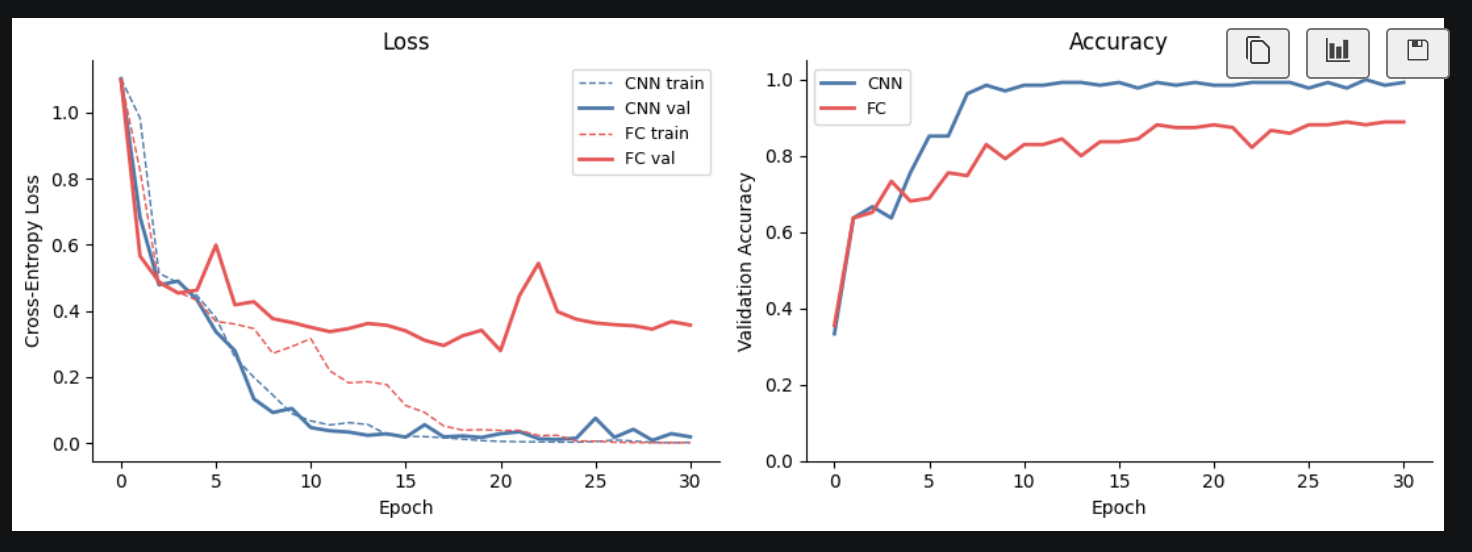
\includegraphics[width=.98\linewidth,trim=18 18 18 18,clip]{figures/CNN_Loss_Accuracy_Curves.png}
	\caption{Baseline CNN vs FC curves: cross-entropy loss (left) and validation accuracy (right).}
	\label{fig:cnn_loss_accuracy_curves}
\end{figure}

These trends indicate that the CNN captured spatial structure more effectively and generalized better, despite using far fewer parameters than the FC model.

\subsection{Architecture Comparison Results}

Figure~\ref{fig:varying_architecture_results} summarizes the results from comparing CNN architectures with different numbers of convolutional layers, filter sizes, and batch-normalization settings.

Several clear patterns appear from this comparison:

\begin{itemize}
	\item The best overall configuration was the 3-layer CNN with filters \texttt{[16, 32, 64]} and no batch normalization, which achieved a test accuracy of 99.3\%.
	\item Very small models, such as the 2-layer \texttt{[8, 16]} network, still performed well, but they did not match the strongest 3-layer model.
	\item Increasing depth from 3 layers to 4 layers did not improve final test accuracy, even when validation accuracy reached 100\%, suggesting diminishing returns from extra depth on this dataset.
	\item Batch normalization did not consistently improve results. In several cases it produced similar or slightly lower test accuracy than the corresponding model without batch normalization.
\end{itemize}

Overall, the architecture comparison suggests that a moderate-depth CNN is sufficient for this task: three convolutional blocks provided the best balance of model capacity and generalization, while more layers or additional normalization did not yield a meaningful accuracy gain.

\begin{figure}[htb]
	\centering
	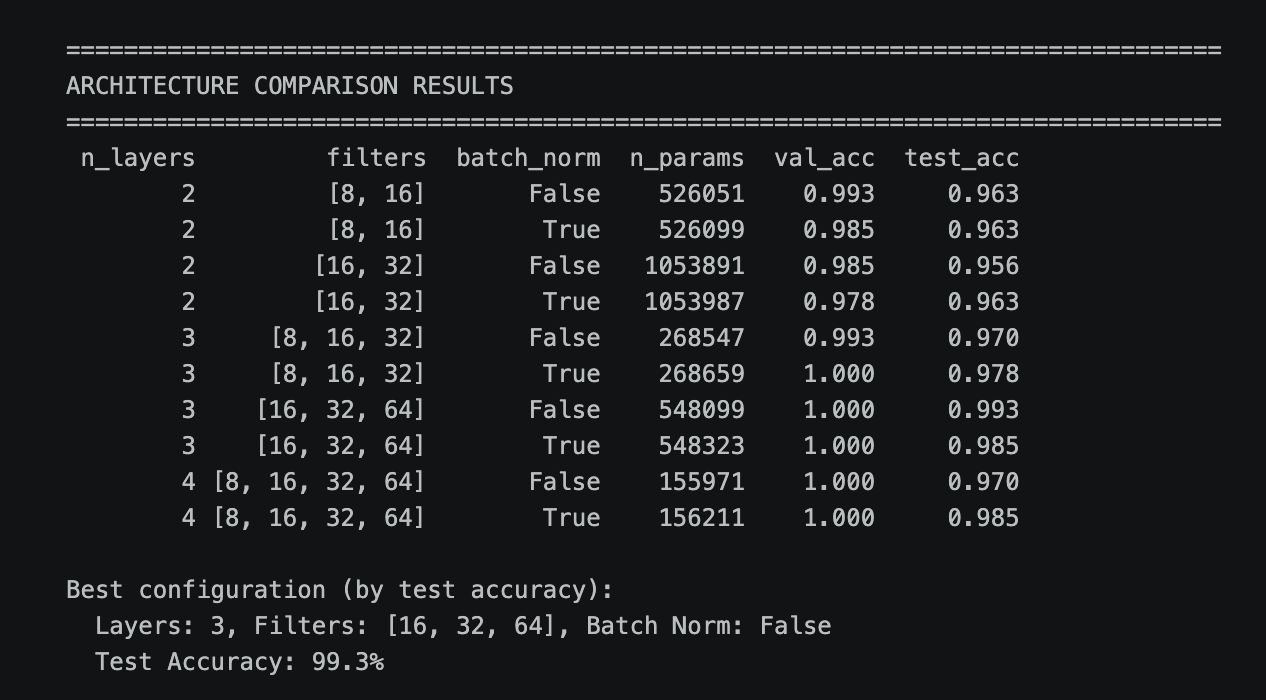
\includegraphics[width=.98\linewidth]{figures/Varying_Architecture_Experiment_Results.png}
	\caption{Comparison of CNN architecture options, including number of layers, filter sizes, parameter counts, and validation/test accuracy.}
	\label{fig:varying_architecture_results}
\end{figure}

\subsection{Regularization Results}

Figure~\ref{fig:regularization_training_vs_accuracy} compares training and validation accuracy with and without regularization.

The main interpretation is based on the train-vs-validation gap:

\begin{itemize}
	\item A larger gap between training accuracy and validation accuracy indicates stronger overfitting.
	\item Effective regularization should reduce this gap while still keeping validation and test accuracy high.
\end{itemize}

From the curves, the unregularized model quickly reached near-perfect training accuracy and also maintained very high validation accuracy, indicating that this dataset is relatively easy for the CNN. The regularized models showed more fluctuation in validation accuracy, but they still remained competitive while controlling the tendency to overfit. This suggests that regularization can improve robustness without sacrificing overall performance, even when the baseline model already performs strongly.

\begin{figure}[htb]
	\centering
	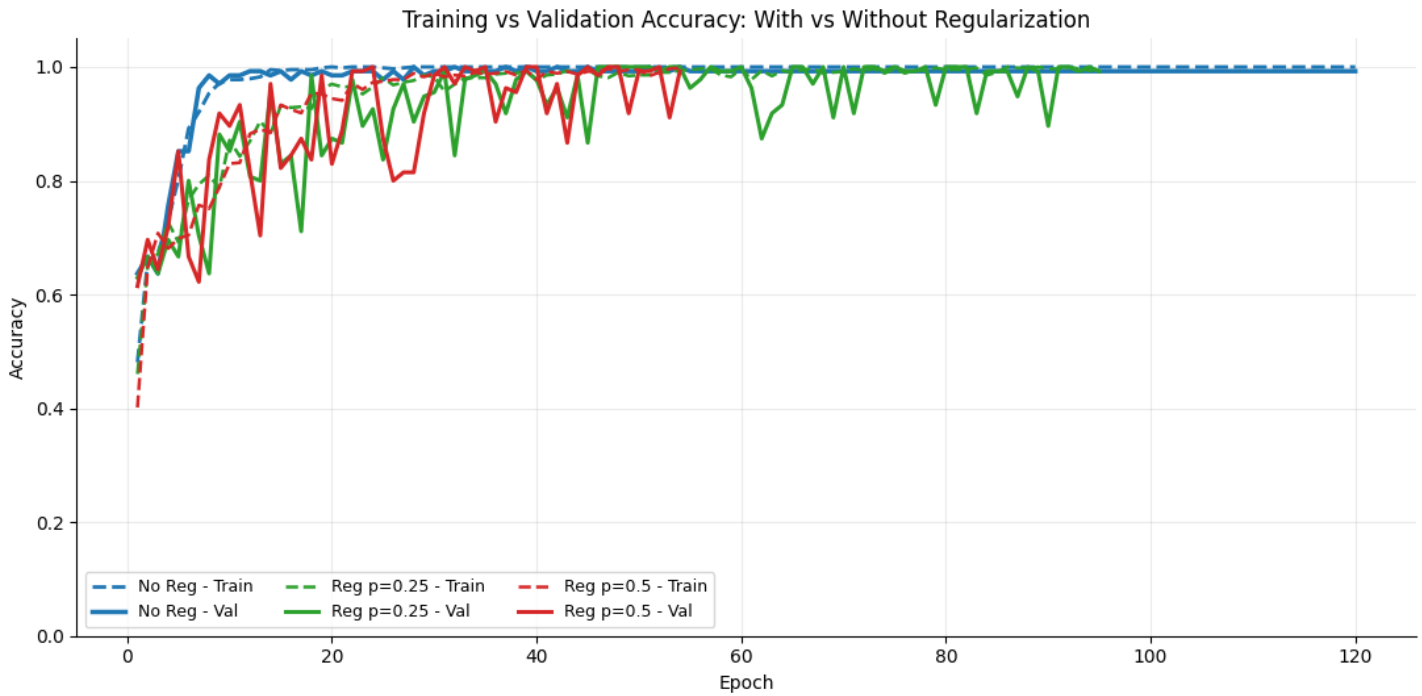
\includegraphics[width=.98\linewidth]{figures/Regularization_Training_vs_Accuracy.png}
	\caption{Training versus validation accuracy for the baseline model and regularized models with dropout. Dashed lines show training accuracy and solid lines show validation accuracy.}
	\label{fig:regularization_training_vs_accuracy}
\end{figure}

\subsection{Held-Out Evaluation of the Best Regularized Model}

After model selection, the best regularized CNN was evaluated on the held-out test set. Figure~\ref{fig:confusion_matrix_best_regularized_model} shows the confusion matrix, and Figure~\ref{fig:held_out_examples_best_regularized_model} shows representative held-out examples.

The confusion matrix is strongly concentrated along the main diagonal, which indicates that the model classified almost all test images correctly. This matches the very high overall test accuracy and shows that the learned representation generalizes well across all three classes.

\begin{itemize}
	\item The diagonal dominance means that normal, damaged, and overloaded shelves were usually separated correctly.
	\item The few remaining mistakes are limited and appear to come from visually similar boundary cases rather than a systematic failure on one class.
	\item In particular, occasional confusion between mildly damaged and normal shelves is reasonable because these cases can share similar loading patterns, with only subtle crack features distinguishing them.
\end{itemize}

The held-out example images reinforce this interpretation. Most examples are classified correctly, while the rare misclassified cases appear close to class boundaries or contain weaker visual cues. Together, these plots show that the best regularized model is both accurate and robust on unseen data.

\begin{figure}[htb]
	\centering
	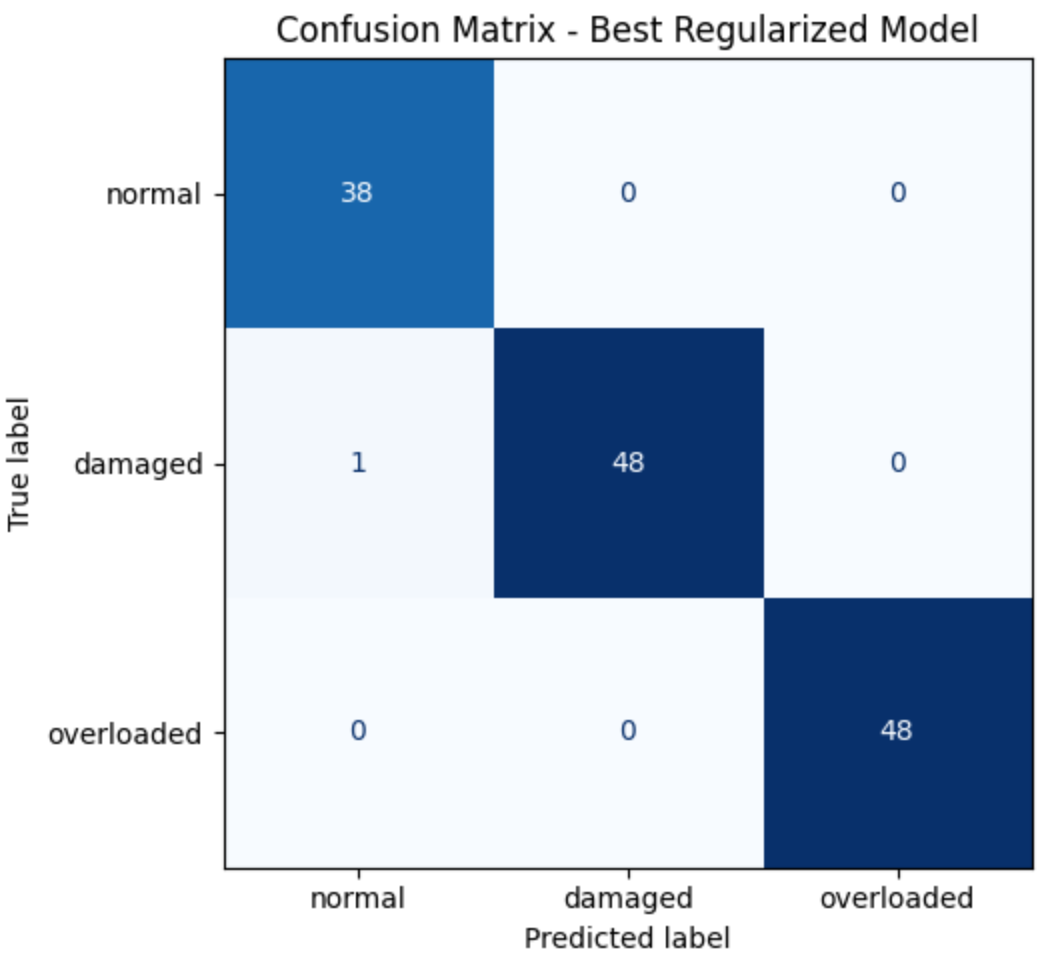
\includegraphics[width=.98\linewidth]{figures/Confusion_Matrix_Best_Regularized_Model.png}
	\caption{Confusion matrix for the best regularized CNN evaluated on the held-out test set.}
	\label{fig:confusion_matrix_best_regularized_model}
\end{figure}

\paragraph{Observations from Figure~\ref{fig:confusion_matrix_best_regularized_model}}
The confusion matrix provides a class-by-class view of model behavior. The high values along the diagonal confirm strong class separation on unseen data, while the small off-diagonal counts indicate that errors are infrequent and localized to borderline examples rather than widespread class confusion.

\begin{figure}[htb]
	\centering
	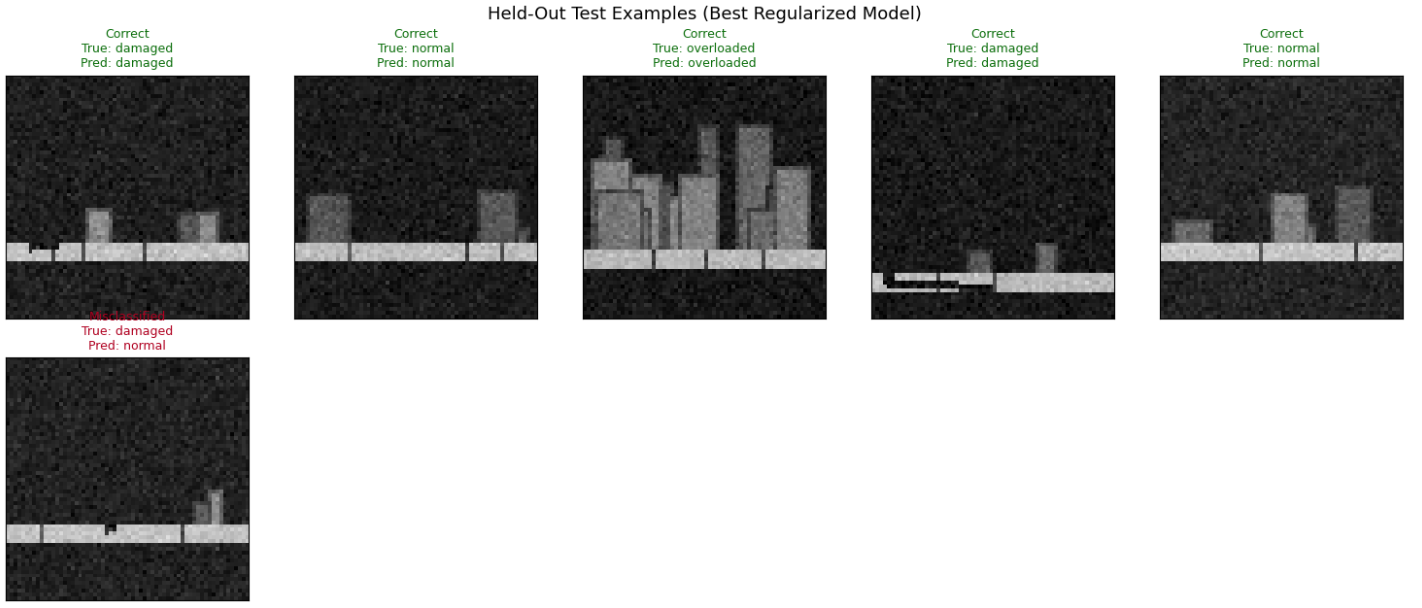
\includegraphics[width=.98\linewidth]{figures/Held-out_Test_Examples_Best_Regularized_Models.png}
	\caption{Representative held-out test examples for the best regularized CNN, including correct predictions and misclassified cases.}
	\label{fig:held_out_examples_best_regularized_model}
\end{figure}

\subsection{Learned First-Layer Filters}

To better interpret what the CNN learns, we visualize first-layer filters for both the baseline CNN (Figure~\ref{fig:learned_first_layer_filters}) and the best regularized CNN (Figure~\ref{fig:best_regularized_first_layer_filters}). These filters operate at the finest spatial scale and reveal local patterns the models use before deeper feature composition.

\begin{itemize}
	\item Edge detectors are clearly present: several filters show opposite signed regions (red vs blue), indicating sensitivity to local intensity transitions.
	\item Orientation-selective patterns appear across the bank: some filters emphasize horizontal and vertical boundaries, while others capture diagonal transitions.
	\item Texture and blob-like responses also emerge: a subset of filters behaves more like local contrast templates than pure edge operators.
	\item Some near-zero filters remain: mostly gray kernels suggest weaker or less frequently used features for this trained model.
\end{itemize}

Overall, these patterns match expected convolutional-network behavior: early layers learn reusable local visual primitives (edges, contrast, and texture) that later layers combine into higher-level class-discriminative representations.

\begin{figure}[htb]
	\centering
	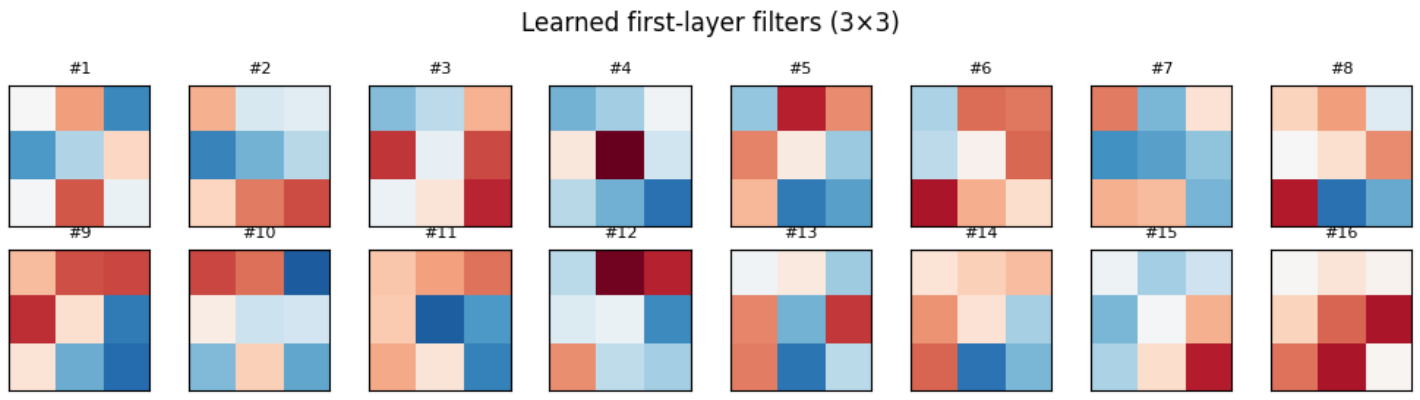
\includegraphics[width=.98\linewidth]{figures/Learned_First_Layer_Filters.png}
	\caption{First-layer convolution filters learned by the baseline CNN model.}
	\label{fig:learned_first_layer_filters}
\end{figure}

\paragraph{Connection to Convolutional Layers}
In convolutional layers, small kernels slide across the input and compute local dot products. This produces feature maps that activate when a learned local pattern is present. Because the same kernel is reused at all spatial positions (weight sharing), the model learns reusable local primitives rather than location-specific templates.

\begin{figure}[htb]
	\centering
	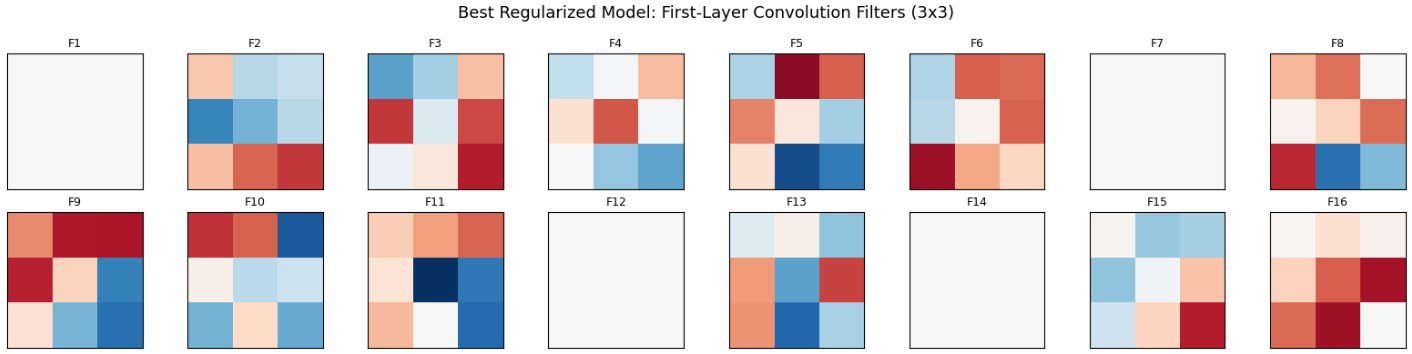
\includegraphics[width=.98\linewidth]{figures/Best_Regularized_Model_First_Layer_Convolution_Filters.png}
	\caption{First-layer convolution filters learned by the best regularized CNN model.}
	\label{fig:best_regularized_first_layer_filters}
\end{figure}

\paragraph{Comparison Between the Two Filter Sets}
Both models learn the same core primitives (edges, orientation-selective patterns, and texture-like responses), but the best regularized model shows a slightly cleaner and more balanced filter bank. Compared with the baseline, its filters appear less dominated by a few high-magnitude kernels and more evenly distributed across orientations, which is consistent with improved generalization. In contrast, the baseline still learns useful detectors, but it can include a few more redundant or high-contrast-specialized kernels. This qualitative difference aligns with the regularization results: regularization does not change \emph{what} the first layer learns, but it can improve \emph{how robustly} those features are represented.

\subsection{Sample Predictions}

Figure~\ref{fig:sample_predictions} compares predictions from the CNN and fully connected models on six held-out test images (two per class: normal, damaged, overloaded).

From these examples, CNN predictions are more consistently correct than the fully connected baseline.

\begin{itemize}
	\item The CNN better preserves class distinctions that depend on local spatial patterns (for example, shelf cracks and dense stacking).
	\item The FC model shows occasional mismatches, especially on visually ambiguous examples where spatial structure is important.
	\item Errors tend to occur on boundary cases, where an image shares traits of two classes (for example, mild damage vs normal, or moderate stacking vs overloaded).
\end{itemize}

Overall, the sample predictions are consistent with the quantitative metrics: convolutional feature extraction improves robustness and class separability for this image-classification task.

\begin{figure}[htb]
	\centering
	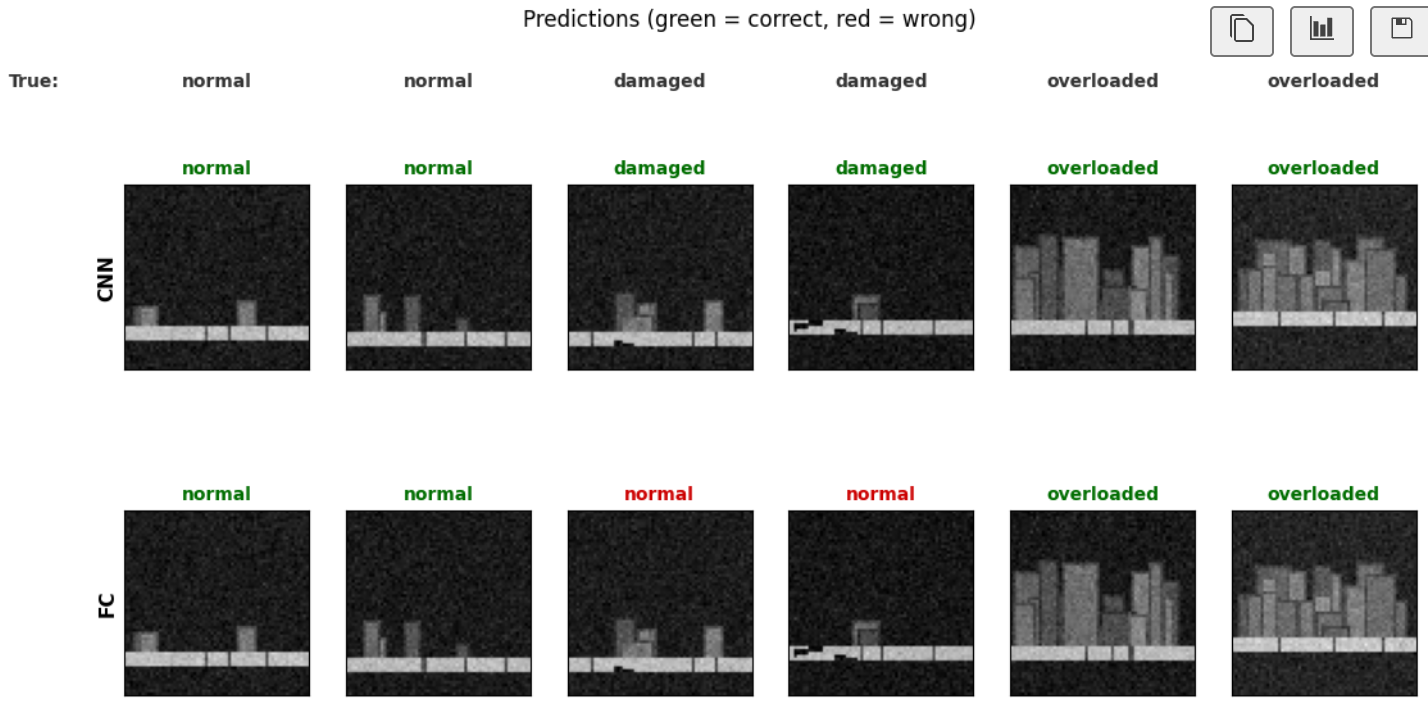
\includegraphics[width=.98\linewidth]{figures/Sample_Predictions.png}
	\caption{Sample held-out predictions for CNN (top row) and fully connected baseline (bottom row). Green labels are correct predictions and red labels are incorrect predictions.}
	\label{fig:sample_predictions}
\end{figure}

\paragraph{Comparison of Figure~5 and Figure~8}
Figure~5 (held-out examples for the best regularized model) shows how the final selected CNN behaves on unseen data after regularization and model selection, with only rare errors on subtle boundary cases. Figure~8 (CNN vs FC sample predictions) highlights the earlier model-family gap, where CNN predictions are more reliable than the fully connected baseline on the same type of visual task. Taken together, these two figures support a consistent conclusion: convolutional feature extraction provides the main performance advantage, and regularization helps make that advantage more robust on difficult test examples.

\paragraph{Qualitative Takeaway}
\begin{itemize}
	\item CNN predictions were more consistently correct across classes.
	\item Learned first-layer filters resembled edge/contrast detectors, matching expected CNN behavior for image tasks.
\end{itemize}

\section{Conclusion}
This experiment showed that convolutional modeling is the right choice for shelf-condition image classification. Across baseline comparison, architecture exploration, and regularization experiments, the CNN consistently outperformed the fully connected baseline while using image-appropriate local feature extraction. The best-performing setup was a 3-layer CNN with filter progression \texttt{[16, 32, 64]}, which achieved strong validation and held-out test performance.

Regularization improved robustness by controlling overfitting without sacrificing accuracy, and held-out evaluation confirmed reliable class separation with only limited boundary-case errors. Finally, first-layer filter visualizations provided interpretable evidence that the model learned meaningful edge-, orientation-, and texture-sensitive detectors, consistent with convolutional-network theory. Overall, the results support the use of a moderately deep, regularized CNN as an effective and generalizable solution for this three-class shelf inspection task.

%%% References -------------------------

\nocite{*}
\bibliographystyle{plainnat}
\bibliography{report}


%%% Appendices -------------------------

\end{document}  